% slides_sim_fakegeo.tex -- cardiac-sim-fakegeo 汇报幻灯片
% 编译:xelatex slides_sim_fakegeo.tex   (需 ctex + fandol,TeX Live 自带)
%       图片 fig_mesh.png / fig_verify_fields.png 与本文件同目录时会自动嵌入。
\documentclass[aspectratio=169,11pt,fontset=fandol]{ctexbeamer}
\usetheme{Madrid}
\usecolortheme{whale}
\usepackage{booktabs}
\usepackage{array}
\usepackage{multirow}
\usepackage{amsmath}
\usepackage{xcolor}
\usepackage{graphicx}
\definecolor{good}{RGB}{22,140,74}
\definecolor{bad}{RGB}{200,38,38}
\definecolor{hl}{RGB}{234,88,12}
\newcommand{\up}{\textcolor{bad}{$\uparrow$}}
\newcommand{\dn}{\textcolor{good}{$\downarrow$}}
\setbeamertemplate{navigation symbols}{}
\setbeamerfont{footline}{size=\tiny}

\title[cardiac-sim-fakegeo]{三系统耦合前向 ECG:真几何 FEM 与 ASM/sASM 区域分解预条件}
\subtitle{分支 \texttt{cardiac-sim-fakegeo} · 算法(数值线性代数 / 区域分解)研究}
\author{tianhaoma-hpc}
\date{MFEM 4.9 + PETSc 3.19 · \texttt{heart.msh} 全部真机实测}

\begin{document}

\begin{frame}\titlepage\end{frame}

\begin{frame}{概览:研究性质与主线}
\textbf{研究性质}:Krylov 预条件 / 区域分解(Additive Schwarz)算法研究。载体是耦合 PDE 前向问题,\emph{对象是线性系统怎么更快收敛、怎么强可扩展}。
\vspace{0.6em}
\begin{block}{管线}
\[
\underbrace{\text{Sys1 } V_m}_{\text{抛物·局部}}\ \xrightarrow{V_m(t)}\
\underbrace{\text{Sys2 } u_e}_{\text{奇异椭圆·全局}}\ \xrightarrow{\text{Dirichlet}}\
\underbrace{\text{Sys3 } \varphi}_{\text{椭圆·非奇异}}\ \to\ \text{ECG}
\]
\end{block}
\textbf{本报告聚焦}:问题定义、网格、以及 \textbf{ASM(BASIC)} 与 \textbf{sASM(scaled/restricted)} 在三系统上的\textbf{迭代数}与\textbf{计算时间}。
\end{frame}

\begin{frame}{问题:三个线性系统的代数刻画}
每个时间步解三个 SPD(半)正定系统(\texttt{heart.msh},Sys2 为 $10085$ 未知量):
\vspace{0.4em}
\begin{table}\small
\begin{tabular}{@{}lllc@{}}
\toprule
系统 & 方程 & 代数类型 & baseline 迭代 \\
\midrule
\textbf{Sys1} $V_m$ & $\left(\tfrac1{\Delta t}M+\tfrac12K\right)V_m=b$ & 抛物 / \textbf{质量主导} / 非奇异 & CG+ICC $\sim$13 \\
\textbf{Sys2} $u_e$ & $K_{\sigma_i+\sigma_e}\,u_e=-K_{\sigma_i}V_m$ & 椭圆 / \textbf{纯 Neumann 奇异} / 全局 & $\sim$82--96 \\
\textbf{Sys3} $\varphi$ & $K_{\sigma_o}\varphi=0$,交界面 Dirichlet & 椭圆 / 非奇异 / 全局 & $\sim$62--66 \\
\bottomrule
\end{tabular}
\end{table}
\vspace{0.3em}
\textbf{Sys2 是唯一难点}(奇异 $+$ 椭圆 $+$ 全局):
\begin{itemize}
\item $K\mathbf{1}=0$,零空间 $=$ 常数 $=$ 一个慢全局模 $\Rightarrow$ RHS 去均值 $+$ \texttt{MatSetNullSpace}(每步 CG 投影掉常模)。
\item 全局椭圆 $\Rightarrow$ 一层区域分解每迭代只传一个子域跳,子域越多越慢(下文核心)。
\end{itemize}
\end{frame}

\begin{frame}{网格:共形非结构四面体(heart-in-torso)}
\begin{columns}[T]
\begin{column}{0.54\textwidth}
\textbf{几何}:心脏 slab $20\times7\times3$ mm 居中嵌入 $50^3$ mm 躯干;交界面 \textbf{conforming}(Gmsh \texttt{BooleanFragments},共享同一组交界面节点)。\\[0.4em]
\textbf{离散}:P1 连续 Galerkin(MFEM 4.9),各向异性 $\sigma$(纤维 $\parallel x$),单位 mm/ms/mV/mS$\cdot$mm$^{-1}$。
\begin{table}\small
\begin{tabular}{@{}lrrr@{}}
\toprule
网格 & 节点(dof) & 四面体 & 边界三角 \\
\midrule
heart & $10\,085$ & $47\,582$ & $9\,510$ \\
torso & $36\,229$ & $206\,647$ & $12\,112$ \\
\midrule
\multicolumn{4}{@{}l}{交界面共享 dof:$4\,757$(coord-matched,partition-independent)}\\
\bottomrule
\end{tabular}
\end{table}
\end{column}
\begin{column}{0.44\textwidth}
\IfFileExists{fig_mesh.png}{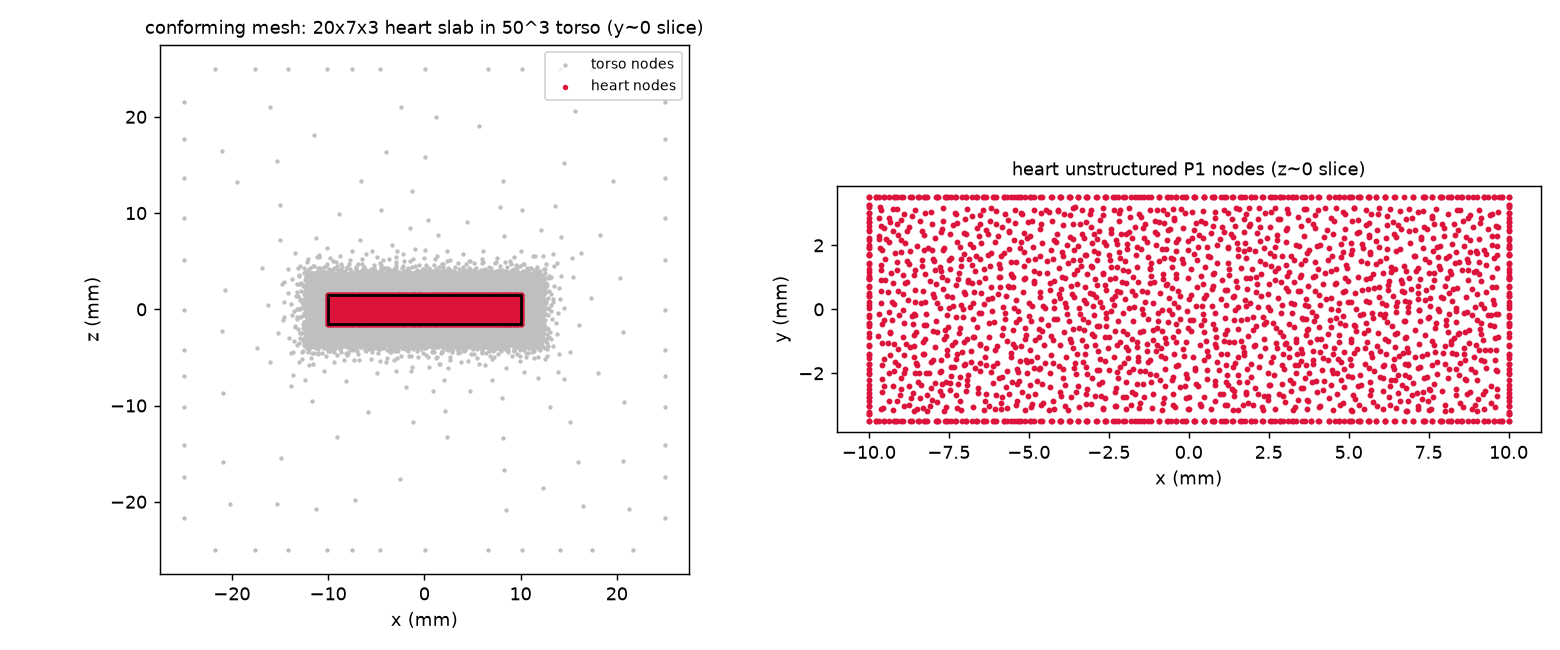
\includegraphics[width=\linewidth]{fig_mesh.png}}%
{\centering\vspace{2em}\fbox{\parbox{0.9\linewidth}{\centering \texttt{fig\_mesh.png}\\(心脏 slab 嵌躯干,$y{\sim}0$ 切片)}}\vspace{2em}}
\end{column}
\end{columns}
\vspace{0.3em}
\footnotesize 子区域 $=$ MPI rank(METIS 几何划分);$n_p{=}$ rank 数 $=$ 子域数。
\end{frame}

\begin{frame}{方法:ASM(BASIC) 与 sASM(scaled / restricted)}
一层加性 Schwarz,子块 $=$ METIS 子域,子解 $=$ ICC(0):
\[
M_{\text{ASM}}^{-1}=\sum_{i} R_i^\top A_i^{-1} R_i,\qquad
A_i=R_i A R_i^\top\ (\text{重叠 } O\text{ 层})
\]
\begin{block}{核心差别 —— 重叠区的\emph{重数(over-count)}}
\begin{itemize}
\item \textbf{ASM(BASIC)}:重叠 dof 被多个子域\emph{各贡献一次} $\Rightarrow$ 重叠处\textbf{过计数},破坏算子谱、甚至\emph{迭代随重叠上升}。
\item \textbf{sASM}:用对角单位分解 $D^{-1/2}(\cdot)D^{-1/2}$ 抵消过计数($D=$ 重数)$\Rightarrow$ 重叠\emph{正常起作用},迭代随重叠下降。
\end{itemize}
\end{block}
\[
M_{\text{sASM}}^{-1}=D^{-1/2}\Big(\textstyle\sum_i R_i^\top A_i^{-1} R_i\Big)D^{-1/2}
\]
$O{=}0$(无重叠)时无过计数,\textbf{ASM $\equiv$ sASM}。
\end{frame}

\begin{frame}{迭代数:ASM vs sASM($n_p{=}4$,rtol $10^{-8}$,ICC(0))}
\begin{table}\small
\begin{tabular}{@{}llccl@{}}
\toprule
系统 & $O$ & ASM(BASIC) & sASM & 备注 \\
\midrule
\multirow{3}{*}{Sys1 $V_m$}
 & 0 & 11 & 11 & $O{=}0$:相等 \\
 & 1 & 13 \up & \textbf{8} \dn & \\
 & 2 & 13 \up & \textbf{8} \dn & \\
\midrule
\multirow{3}{*}{Sys2 $u_e$(奇异)}
 & 0 & 82 & 82 & \\
 & 1 & 92 \up & \textbf{74} \dn & \\
 & 2 & 93 \up & \textbf{74} \dn & \\
\midrule
\multirow{3}{*}{Sys3 $\varphi$}
 & 0 & 62 & 62 & \\
 & 1 & 88 \up & \textbf{53} \dn & \\
 & 2 & 94 \up & \textbf{53} \dn & \\
\bottomrule
\end{tabular}
\end{table}
\vspace{-0.3em}
\footnotesize \textcolor{bad}{$\uparrow$ ASM 迭代随重叠\emph{上升}}(过计数);\textcolor{good}{$\downarrow$ sASM 随重叠\emph{下降}}(重叠正常生效)。
\end{frame}

\begin{frame}{迭代数:ASM vs sASM($n_p{=}8$,更多子域 $\Rightarrow$ 异常更明显)}
\begin{table}\small
\begin{tabular}{@{}llccl@{}}
\toprule
系统 & $O$ & ASM(BASIC) & sASM & 备注 \\
\midrule
\multirow{3}{*}{Sys1 $V_m$}
 & 0 & 13 & 13 & \\
 & 1 & 18 \up & \textbf{8} \dn & \\
 & 2 & 19 \up & \textbf{8} \dn & \\
\midrule
\multirow{3}{*}{Sys2 $u_e$(奇异)}
 & 0 & 79 & 79 & \\
 & 1 & 117 \up & \textbf{73} \dn & \\
 & 2 & 123 \up & \textbf{71} \dn & \\
\midrule
\multirow{3}{*}{Sys3 $\varphi$}
 & 0 & 66 & 66 & \\
 & 1 & 93 \up & \textbf{55} \dn & \\
 & 2 & 109 \up & \textbf{53} \dn & \\
\bottomrule
\end{tabular}
\end{table}
\vspace{-0.3em}
\footnotesize 最极端:Sys3 ASM $O{:}0{\to}2$ \textcolor{bad}{$66{\to}93{\to}109$($+65\%$)};sASM \textcolor{good}{$66{\to}55{\to}53$($-20\%$)}。
\end{frame}

\begin{frame}{计算时间:ASM vs sASM(ms,KSP+PCASM 建立$+$求解,$20$ 次均值)}
\begin{columns}[T]
\begin{column}{0.5\textwidth}
\centering $n_p=4$\\[0.2em]
\begin{table}\scriptsize
\begin{tabular}{@{}llrr@{}}
\toprule
系统 & $O$ & ASM & sASM \\
\midrule
\multirow{3}{*}{Sys1}&0&3.66&3.79\\&1&5.27&\textbf{5.60}\\&2&6.88&\textbf{5.22}\dn\\
\midrule
\multirow{3}{*}{Sys2}&0&15.39&18.85\\&1&21.50&\textbf{17.60}\dn\\&2&24.33&\textbf{19.39}\dn\\
\midrule
\multirow{3}{*}{Sys3}&0&43.59&46.99\\&1&68.10&\textbf{44.36}\dn\\&2&80.18&\textbf{52.57}\dn\\
\bottomrule
\end{tabular}
\end{table}
\end{column}
\begin{column}{0.5\textwidth}
\centering $n_p=8$\\[0.2em]
\begin{table}\scriptsize
\begin{tabular}{@{}llrr@{}}
\toprule
系统 & $O$ & ASM & sASM \\
\midrule
\multirow{3}{*}{Sys1}&0&5.37&5.62\\&1&8.93&\textbf{7.89}\dn\\&2&14.90&\textbf{8.91}\dn\\
\midrule
\multirow{3}{*}{Sys2}&0&24.48&26.73\\&1&45.72&\textbf{28.94}\dn\\&2&53.15&\textbf{32.83}\dn\\
\midrule
\multirow{3}{*}{Sys3}&0&72.98&59.58\dn\\&1&96.81&\textbf{71.03}\dn\\&2&133.24&\textbf{77.17}\dn\\
\bottomrule
\end{tabular}
\end{table}
\end{column}
\end{columns}
\vspace{0.2em}
\footnotesize $O{\ge}1$ 时 sASM \textbf{迭代更少且墙钟更快};重叠对 ASM 是\emph{赔了时间又涨迭代}。$n_p{=}8$ Sys3 $O{=}2$:ASM $109$it$/133$ms vs sASM $53$it$/77$ms($\sim1.7\times$)。
\end{frame}

\begin{frame}{关键发现:重叠反常(overlap anomaly)}
\begin{block}{现象}
一层 \textbf{ASM(BASIC)} 加重叠,\emph{迭代数不降反升}、墙钟更慢;\textbf{sASM} 加重叠则迭代与墙钟\emph{双降}。
\end{block}
\begin{block}{机理:重叠反常 $=$ 过计数 $\times$ 不精确}
\begin{itemize}
\item 重叠 dof 被多子域各计一次 $\Rightarrow$ BASIC 预条件在重叠区\textbf{放大}($\|M^{-1}\|$ 偏大),谱恶化。
\item ICC(0) 子解\emph{不精确},放大误差不被本地精解吸收 $\Rightarrow$ 迭代升。
\item sASM 的 $D^{-1/2}$ 单位分解精确抵消过计数 $\Rightarrow$ 恢复"重叠越多、信息传播越快"的正常行为。
\end{itemize}
\end{block}
\textbf{结论}:真实几何 FEM 上,\textbf{scaled/restricted ASM 是重叠区域分解的正确用法};BASIC 的重叠在此设置下有害。子域越多($n_p{:}4{\to}8$)反常越强,凸显\emph{可扩展性}需要正确的加权(以及后续的粗空间)。
\end{frame}

\begin{frame}{小结与展望}
\begin{itemize}
\item \textbf{问题}:三系统耦合前向 ECG,Sys2(奇异纯 Neumann 椭圆)是唯一难点、也是预条件研究目标。
\item \textbf{网格}:conforming 非结构四面体 P1-FEM,heart $10085$ dof / $47582$ tets,torso $36229$ / $206647$。
\item \textbf{ASM vs sASM}(真机 $n_p{=}4,8$):
  \begin{itemize}
  \item ASM(BASIC) 迭代\textcolor{bad}{随重叠上升}(过计数),墙钟更慢;
  \item sASM 迭代\textcolor{good}{随重叠下降},$O{\ge}1$ 墙钟也更快;
  \item $O{=}0$ 二者相等。
  \end{itemize}
\item \textbf{下一步}(已在同分支实现/规划):强 fine level \textbf{SORAS}($84{\to}20$,$4.2\times$)、共享 \textbf{Nicolaides 粗空间}(可扩展性)、跨时间 \textbf{Fischer}($-12\%$);大规模($\sim$3000 核)需 \textbf{GenEO 谱粗空间} $+$ telescope 可扩展粗解。
\end{itemize}
\vspace{0.4em}
\centering\footnotesize 全部数字容器内实测(MFEM 4.9 + PETSc 3.19);ECG 逐位不变已核对。
\end{frame}

\end{document}
